% GNUPLOT: LaTeX picture with Postscript
\begingroup
  \makeatletter
  \providecommand\color[2][]{%
    \GenericError{(gnuplot) \space\space\space\@spaces}{%
      Package color not loaded in conjunction with
      terminal option `colourtext'%
    }{See the gnuplot documentation for explanation.%
    }{Either use 'blacktext' in gnuplot or load the package
      color.sty in LaTeX.}%
    \renewcommand\color[2][]{}%
  }%
  \providecommand\includegraphics[2][]{%
    \GenericError{(gnuplot) \space\space\space\@spaces}{%
      Package graphicx or graphics not loaded%
    }{See the gnuplot documentation for explanation.%
    }{The gnuplot epslatex terminal needs graphicx.sty or graphics.sty.}%
    \renewcommand\includegraphics[2][]{}%
  }%
  \providecommand\rotatebox[2]{#2}%
  \@ifundefined{ifGPcolor}{%
    \newif\ifGPcolor
    \GPcolortrue
  }{}%
  \@ifundefined{ifGPblacktext}{%
    \newif\ifGPblacktext
    \GPblacktexttrue
  }{}%
  % define a \g@addto@macro without @ in the name:
  \let\gplgaddtomacro\g@addto@macro
  % define empty templates for all commands taking text:
  \gdef\gplbacktext{}%
  \gdef\gplfronttext{}%
  \makeatother
  \ifGPblacktext
    % no textcolor at all
    \def\colorrgb#1{}%
    \def\colorgray#1{}%
  \else
    % gray or color?
    \ifGPcolor
      \def\colorrgb#1{\color[rgb]{#1}}%
      \def\colorgray#1{\color[gray]{#1}}%
      \expandafter\def\csname LTw\endcsname{\color{white}}%
      \expandafter\def\csname LTb\endcsname{\color{black}}%
      \expandafter\def\csname LTa\endcsname{\color{black}}%
      \expandafter\def\csname LT0\endcsname{\color[rgb]{1,0,0}}%
      \expandafter\def\csname LT1\endcsname{\color[rgb]{0,1,0}}%
      \expandafter\def\csname LT2\endcsname{\color[rgb]{0,0,1}}%
      \expandafter\def\csname LT3\endcsname{\color[rgb]{1,0,1}}%
      \expandafter\def\csname LT4\endcsname{\color[rgb]{0,1,1}}%
      \expandafter\def\csname LT5\endcsname{\color[rgb]{1,1,0}}%
      \expandafter\def\csname LT6\endcsname{\color[rgb]{0,0,0}}%
      \expandafter\def\csname LT7\endcsname{\color[rgb]{1,0.3,0}}%
      \expandafter\def\csname LT8\endcsname{\color[rgb]{0.5,0.5,0.5}}%
    \else
      % gray
      \def\colorrgb#1{\color{black}}%
      \def\colorgray#1{\color[gray]{#1}}%
      \expandafter\def\csname LTw\endcsname{\color{white}}%
      \expandafter\def\csname LTb\endcsname{\color{black}}%
      \expandafter\def\csname LTa\endcsname{\color{black}}%
      \expandafter\def\csname LT0\endcsname{\color{black}}%
      \expandafter\def\csname LT1\endcsname{\color{black}}%
      \expandafter\def\csname LT2\endcsname{\color{black}}%
      \expandafter\def\csname LT3\endcsname{\color{black}}%
      \expandafter\def\csname LT4\endcsname{\color{black}}%
      \expandafter\def\csname LT5\endcsname{\color{black}}%
      \expandafter\def\csname LT6\endcsname{\color{black}}%
      \expandafter\def\csname LT7\endcsname{\color{black}}%
      \expandafter\def\csname LT8\endcsname{\color{black}}%
    \fi
  \fi
  \setlength{\unitlength}{0.0500bp}%
  \begin{picture}(7200.00,5040.00)%
    \gplgaddtomacro\gplbacktext{%
    }%
    \gplgaddtomacro\gplfronttext{%
      \csname LTb\endcsname%
      \put(3853,724){\makebox(0,0)[r]{\strut{}max. Tiefe}}%
      \csname LTb\endcsname%
      \put(2426,1140){\makebox(0,0){\strut{}-100}}%
      \put(2555,1103){\makebox(0,0){\strut{}-50}}%
      \put(2683,1066){\makebox(0,0){\strut{} 0}}%
      \put(2812,1029){\makebox(0,0){\strut{} 50}}%
      \put(2941,992){\makebox(0,0){\strut{} 100}}%
      \put(3069,955){\makebox(0,0){\strut{} 150}}%
      \put(3198,918){\makebox(0,0){\strut{} 200}}%
      \put(3326,881){\makebox(0,0){\strut{} 250}}%
      \put(3455,843){\makebox(0,0){\strut{} 300}}%
      \put(2710,830){\makebox(0,0){\strut{}x [m]}}%
      \put(3578,911){\makebox(0,0){\strut{}-700}}%
      \put(3726,1040){\makebox(0,0){\strut{}-600}}%
      \put(3874,1168){\makebox(0,0){\strut{}-500}}%
      \put(4023,1297){\makebox(0,0){\strut{}-400}}%
      \put(4171,1426){\makebox(0,0){\strut{}-300}}%
      \put(4320,1554){\makebox(0,0){\strut{}-200}}%
      \put(4468,1683){\makebox(0,0){\strut{}-100}}%
      \put(4617,1811){\makebox(0,0){\strut{} 0}}%
      \put(4765,1940){\makebox(0,0){\strut{} 100}}%
      \put(4371,1379){\makebox(0,0){\strut{}y [m]}}%
      \put(2366,1922){\makebox(0,0)[r]{\strut{}-2.5}}%
      \put(2366,2196){\makebox(0,0)[r]{\strut{}-2}}%
      \put(2366,2470){\makebox(0,0)[r]{\strut{}-1.5}}%
      \put(2366,2744){\makebox(0,0)[r]{\strut{}-1}}%
      \put(2366,3018){\makebox(0,0)[r]{\strut{}-0.5}}%
      \put(2366,3292){\makebox(0,0)[r]{\strut{} 0}}%
      \put(1568,2608){\makebox(0,0){\strut{}z [m]}}%
    }%
    \gplbacktext
    \put(0,0){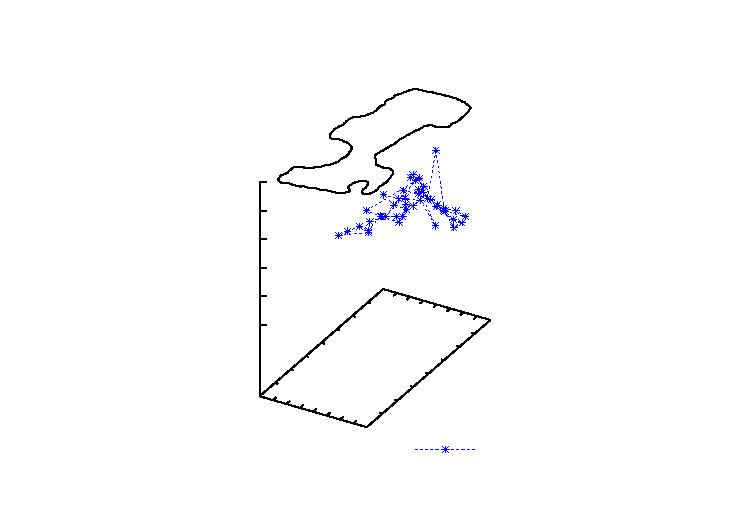
\includegraphics{tiefeGoe}}%
    \gplfronttext
  \end{picture}%
\endgroup
